\documentclass{article}
\usepackage[utf8]{inputenc}

\usepackage{listings}
\usepackage{ntheorem}
\usepackage{lipsum}

\newtheorem{theorem}{Theorem}
\usepackage{float}
\usepackage{amssymb} 
\usepackage[letter, margin=1in]{geometry}
\usepackage{natbib}
\usepackage{graphicx}
\usepackage{amsmath}



% correct bad hyphenation here
\hyphenation{op-tical net-works semi-conduc-tor}


\begin{document}
\title{Linear System Analysis\\Final Porject}
\author{Jian Chu (jc86537)}
\markboth{ASE 381P, November~2019}%
{Shell \MakeLowercase{\textit{et al.}}: Bare Demo of IEEEtran.cls for IEEE Journals}
\maketitle

\section{Part A}
In this part we will focus on the "slowly varying" system. Since the parameters are changing very slowly, we will intuitively expect that the system can be predicted by some specific "frozen" time. If this is true, we can use some convenient method to analyze this kind of system, such as calculating the eigenvalues. However, there are many famous counterexamples for this idea. Therefore, many research focus on the criterion of how to check the system is stability or not. The system used in the follow review mostly is $\dot{x} = A(t)x$, we will take this as our default system.

\subsection{Instability of Slowly Varying System \cite{skoog1972instability}}
Let us start from the LTI system, for LTI system to be stable, generally we need the matrix to be Hurwitz, in the other words, all the eigenvalues of $A$ should lie on the open left half plane. We know that it is not true for time varying system, even if all eigenvalues strictly stay in the open left half plane, the system still can be unstable. However, the opposite conclusion is still wrong, this paper gave us an example to show that even if there are eigenvalues stay in the open right half plane, the system still can be stable. In another words, whether the system is stable will not depend on the location of the eigenvalues directly. We need to find when we can apply the result from time invariant system to this kind of system. Or we need more assumptions to claim whether the system is stable or not. 

It is well known that: 

1. If the eigenvalues of $A(t)$ lie in $Re \lambda < \sigma_0 < 0$ for all $t$ 

2. $\sup_{t \ge 0} ||\dot{A}(t)||$ is sufficient small

then all solutions of $\dot{x}=A(t)x$ go to zero as $t \rightarrow \infty$. Particular the paper is shown that, the opposite conclusion is true. That, when $A(t)$ has eigenvalues in the right-half plane and all eigenvalues are bounded away from the imaginary axis, then if $\sup_{t \ge 0}||\dot{A}(t)||$ is sufficiently small, the system has unbounded all solutions. But, the example in this paper showed us it is not the necessary condition. 

In Section III the author showed that, if the eigenvalues are allowed to cross the imaginary axis, then even though there is always an eigenvalue with positive real part, the system can be asymptotically stable for arbitrarily
small $\sup_{t \ge 0} ||\dot{A}(t)||$. This result also holds for nonlinear systems of form $\dot{x} = A(t)x + f(x,t)$ where $||f(x,t)||/||x|| \longrightarrow 0$ as $||x|| \longrightarrow 0$

So it means the intuitive conclusion for system stability can be relaxed somehow. Notice the example $II$ here, the author shows that the stability does not comes from the equality of these two eigenvalues. (The example he gave, two eigenvalues may be equal in sometimes, so he gave a more general example)

This paper's proof is similar to the other three papers which using Lyapunov methods, however, we cannot construct the same Lyapunov function due to the eigenvalues (both left and right). The tricky part of this paper is the author divided the eigenvalues to two sets for some eigenvalues lie on the right half plane and never cross the imaginary axis. Then use the decomposition theorem (Section II) we can re-construct the Lyapunov function with 

$$v(z,t)=z^T Q v \ where \ T(t)z(t)=x(t), Q = diag\{Q_1,Q_2\}$$
$$A_1^T Q_1 + Q_1 A_1 = -I_{k \times k}, A_2^T Q_2 + Q_2 A_2 = -I_{(n-k) \times (n-k)}$$ 

Actually this is a kind of transformation of state $x$. Then we can give the upper bound of terms of $\dot{v}(t)$ to show $\dot{v}(t) \leq -\gamma z^T(t) z(t)$ for some $\gamma > 0$ if $\dot{\alpha} < \frac{1}{c}$. Which is unstable due to the Lyapunov Theorem. Then, for $\dot{x} = A(t)x + f(x,t)$, it is also unstable (No Proof in the paper).

In the Time-Invariant case, we know that, if the matrix $A$ has $k$ eigenvalues with negative real parts, then for the system $\dot{x}(t) = Ax(t)$ there exists a $k$-dimensional subspace of $R^n$ such that, if $\phi(t)$ is a solution of these equation with $\phi(t_0)$ in this subspace, then $||\phi(t)|| \leq \alpha e^{-\sigma(t-t_0)}$ for some constants $\alpha,\sigma > 0$, and it is true for $\dot{x} = A(t)x + f(x,t)$. For slowly varying system, these result also holds!

In summary, this paper showed us a counter-example and prove the unstable for non-crossing imaginary axis case. Also showed some result keep the same when the system changes from the TI to Slowly Varying case. However, the assumptions in this paper is too strong, especially eigenvalues cannot cross the imaginary axis. In the other papers\cite{solo1994stability}, we will relax this assumption.

\subsection{Sufficient Conditions for Stability of Linear Time-Varying Systems\cite{ilchmann1987sufficient}}
\indent This paper analyze exponential stability for the systems of the form $$\dot{x}=A(t)x(t), t \ge 0, A(\cdot): R_{+} \rightarrow R^{n \times n}$$ 

It is usually a priori required that $A(\cdot)$ belongs to the set $\mathcal{F}$ of all piecewise continuous matrix functionsis which satisfies:

1. There exist $M>0$ such that $||A(t)|| \leq M$ for all $t \ge 0$

2. There exist $\alpha>0$ such that the eigenvalues of $A(t)$ are contained in $C^{-\alpha} = \{s \in C | Re \ s \leq -\alpha \}$ for all $t \ge 0$

It is known that for time invariant system, the assumptions are enough to claim stability. But not for time variant system, from some examples we found that, if want to conclude exponentially stable, we need have additional restrictions on variation of the element of $A(\cdot)$. Many researchers gave their criterions, some assumption may be easy to check but not necessary, some maybe very accurate but not easy to use, some may focus on the mathematical meaning but not very useful in practice. Therefore, we want to compare these assumptions to analyze their advantages and disadvantages. In this paper, the author proposed some "suitable" assumptions and gave the explicit formulas for parameter variation upper bound. 

In the previous research, if $\delta > 0$ is sufficient small, the assumptions to make the slowly varying system to be exponential stable include:

1. $||\dot{A}(t)||\leq \delta$ for all $t > 0$

2. $||A(t_2)-A(t_1)||\leq \delta ||t_2 - t_1||$, for all $t_1,t_2 \geq 0$

3. $\sup\limits_{0\leq \tau \leq h}||A(t+\tau)-A(t)||\leq \delta$ for some $h>0$

4. $\dot{A}(\cdot)$ is continuous, $||\dot{A}(\cdot)||$ is uniformly bounded and there exists $T>0$ such that $\int_{t_0}^{t_0+T} {||\dot{A}(t)||}\leq \delta T$ for all $t_0 \geq 0$

5.$\lim\limits_{t\rightarrow \infty} \sup\limits_{0\leq \tau \leq h}||A(t+\tau)-A(t)|| = 0 $ for all $h>0$

Based on the above assumptions, we all can claim exponential stability if $\delta > 0$ is sufficient small. But how we can use this in practice? What is "sufficient small" mean? The author gave two theorem to claim the "sufficient small" and gave the upper bound for the parameters.

\begin{figure}[H]
\centering
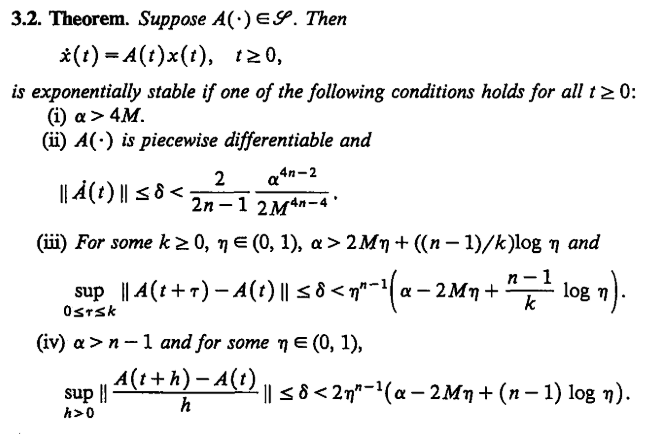
\includegraphics[width=0.5\linewidth]{Ref_2_Theorem_1.png}
\caption{Theorem 1 for "sufficient small"}
\end{figure}

Let's consider each condition. The first condition is easiest and simplest way to check. Since $M \ge ||A(t)||$ and $\alpha = |Re \lambda(A(t))|$, thus, $\alpha$ should be less than $M$ in most cases. The second condition is less restrictive, but we noticed that $\alpha$ is usually less than $M$, thus, the bound $\delta$ will decrease exponentially as the $n$ grows. The third and fourth condition are similar, they do not ask for differentiable condition but add some restriction here.

\begin{figure}[H]
\centering
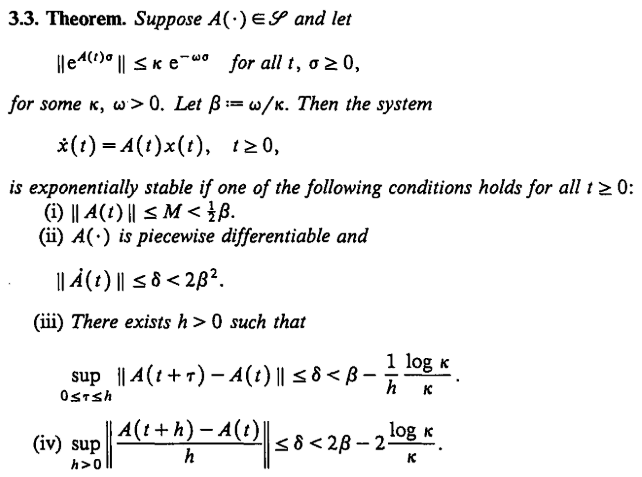
\includegraphics[width=0.5\linewidth]{Ref_2_Theorem_2.png}
\caption{Theorem 2 for "sufficient small"}
\end{figure}

The author make the theorem simpler to use based on some known information and generate theorem 2 here. Obviously when we have more information about the system, it will be easier for us to check the stability properties. 

In summary, in this paper the author concluded the previous results which  guaranteed exponential stability for slowly varying systems and make some improvements on proof for assumption 4. The most significant thing in the paper is that based on these assumptions, the author gave the explicit upper bound for the "sufficient small" parameters, which has much more practical meaning.

\subsection{Slowly-Varying $\dot{x} = A(t)x$\cite{desoer1969slowly}}
This paper is the earliest one among these four papers, and "its assumptions have become more or less standard" for the future research. We can easily find some highlights from the other three papers are based on his assumptions. In this paper, he firstly prove the conditions to establish exponential stability of "slowly varying" system. In addition, his methods to analyze the system also inspired other researchers. We can notice that the methods in the other paper are more or less come from here. I will mention that in the review of other papers.

It starts with the Rosenbrock's theorem:\\
\begin{figure}[H]
\centering
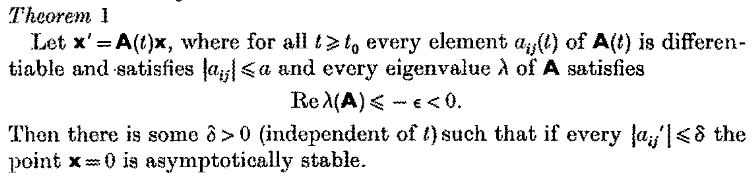
\includegraphics[width=0.7\linewidth]{Ref_3_Theorem_1.png}
\caption{Theorem}
\end{figure}
% if $A(t)$ is differentiable and staisfies $|a_{i j}| \leq a$ (1) and every eigenvalue $\lambda$ of $A$ satisfies $Re \lambda (A) \leq -\epsilon < 0$ (2), then there is some $\delta > 0$ such that if every $|\dot{a}_{i j}| \leq \delta$ the point $x=0$ is asymptotically stable.

Based on this theorem, Desoer gave a bound for $\sup_{t \ge 0} ||\dot{a_M}||$ (which is equivalent to $|a_{i j}^{'}|$ in the theorem) to conclude exponential stable. His assumptions are:

(1*). If the function $t \rightarrow A(t)$ is a matrix-valued piecewise continuous function bounded on $R_{+}$, $a_M \triangleq \sup_{t \ge 0} ||A(t)|| < \infty$ 

(2*). If there is a $\sigma_0 > 0$ $s.t.$ $Re \lambda_i[A(t)] \leq -2 \sigma_0 < 0, \forall i. \forall t \ge 0$ 

Here the assumption (1*) and (2*) are corresponding to assumptions (1) and (2) from Rosenbrock. And under (1*) and (2*), he proved $||e^{A(t) \tau}|| \leq \beta R k^{n-1} / \sigma_0^n \cdot e^{-\sigma_0 \tau} = m e^{-\sigma_0 \tau}$, and the constant $m = \beta R k^{n-1} / \sigma_0^n$ depends only on $\sigma_0$ and $a_M$.Thus,

(3*). $||e^{\tau A(t)}|| \leq m e^{-\sigma_0 \tau}, \forall \tau \ge 0$ .

For proving (3*), he used Cauchy Integral which is widely used in other's future research. It is very useful to get a bound for some norm of matrices. His proof comes as follows: from (1*) and (2*), we know the eigenvalue $\lambda_i$ is bounded, let $|\lambda_i| \leq R/2, \forall i, \forall t \ge 0$, then consider the Laplace transform inversion, $e^{A(t) \tau} = \frac{1}{2 \pi j} \int_C [s I - A(t)]^{-1} e^{s \tau} ds$, take the norm, $||e^{A(t) \tau}|| \leq ||\frac{1}{2 \pi j}|| \beta \int_C \frac{||s I - A(t)||^{n-1}}{|det[s I - A(t)]|} ||e^{s \tau}|| ds \leq \frac{\beta}{2 \pi} e^{-\sigma_0 \tau} \int_C \frac{||s I - A(t)||^{n-1}}{|det[s I - A(t)]|} ds \leq \frac{\beta}{2 \pi} e^{-\sigma_0 \tau} 2 \pi R k^{n-1} \sigma_0^n = \beta R k^{n-1} / \sigma_0^n \cdot e^{-\sigma_0 \tau}$

Under these three conditions, we can generate a possible Lyapunov function $V(x,t) = x^T (\epsilon_1 I + P(t)) x$ where $\epsilon_1 > 0$. Therefore, $V$ is clearly positive definite. Then he tried to make (4*) $\dot{V} \leq -x^T x$ .
$$\dot{V}(x) = \dot{x}^T (\epsilon_1 I + P(t))x + x^T \dot{P}(t) x + x^T (\epsilon_1 I + P(t)) \dot{x} = x^T(A^T P + PA)x + \epsilon_1 x^T (A^T + A) x + x^T \dot{P} x$$

The tricky step here is letting $A^T(t) P(t) + P(t) A(t) = -3 I$, by picking such $P$, we can get a upper bound for $\dot{P}$: $\dot{P}(t) = \int_0^{\infty} e^{\tau A^T(t)} [\dot{A^T}(\tau)P(\tau) + P(\tau) \dot{A(\tau)}]e^{\tau A(t)}d\tau \Longrightarrow ||\dot{P(t)}|| \leq \dot{a_M} 3 m^4 (2\sigma_0)^{-2}$, Thus $\dot{V}$ is bounded by the product of a scalar and $x^T x$: $\dot{V} \leq x^T x [-3 + 2\epsilon_1 a_M + \dot{a_M} 3 m^4 (2\sigma_0)^{-2}]$, by picking small enough $0 < \epsilon_1 \leq 1/(2 a_M)$ and $\dot{a_M} \leq 4 \delta_0^2 /(3 m^4)$, we can get (4*). Thus, we can conclude exponentially stable.

In summary, we have already known that the key point for stability is the "changing rate" of $A$, which is $||\dot{a}_M||$, from Rosenbrock's theorem. This paper based on the assumptions which make the system asymptotic stable, generate a bound for $||\dot{a}_M||$ to claim exponentially stable. From this result, there are many research on how to make this bound much more precise or achieving the same stability by changing some assumptions. 

\subsection{On the Stability of Slowly Time-Varying Linear Systems\cite{solo1994stability}}

This paper discussed the stability for the "slowly varying" system in both deterministic and stochastic cases. The condition for eigenvalues is less restrictive, it allowed the eigenvalues of $A(t)$ to wander into the right half plane as long as "on average" they are in the left half plane, which is very counter intuitive and interesting.

For the  previous research on the time-varying linear system $\dot{x}(t) = A(t)x(t), t \ge 0$
where $x(t)$ is a $p$-vector and $A(t)$ varies slowly. If we want to make this system stable, usually we have the following three assumptions \cite{rosenbrook1963stability} \cite{desoer1969slowly}:
\begin{itemize}
    \item $||A(t)|| \leq A < \infty$
    \item $||\dot{A}(t)|| \leq A < \infty$
    \item All eigenvalues of $A(t)$ have real part $\leq -\sigma < 0$
\end{itemize}

Based on these assumptions, we can generate $||e^{A(\tau)t}|| \leq M e^{-\alpha t}$ from the first two assumptions, then show the exponentially stable if $\dot{A}$ is small enough. Then, many researchers gave some constraints for the parameter, the best result is $\dot{A} < \sigma^2 / (4M \ln{M})^2$ (for $\alpha$ and $M$ given in (2)). In this paper, the author relaxed the last assumption and showed us the system still can be stable. As I mentioned before, this research also based on Desoer's work \cite{desoer1969slowly} but changed some assumptions.

Let recall the proof process in \cite{desoer1969slowly}, Desoer use Cauchy Integral to generate a bound for a exponential norm, then use Laypunov method to claim stability, in the end used exponential bound to get $|x(t)| \leq \beta |x(t_0)| e^{-\alpha (t-t_0)}$. Following this process, the author also gave an exponential bound:
$$\forall \epsilon > 0, ||e^{A(\tau)t}|| \leq M_{\epsilon}^{'} e^{[\alpha(\tau)+\epsilon ||A(\tau)||]t}, for \ all \ \tau, t \ge 0,$$
$$M_{\epsilon}^{'} = 3(1+2/ \epsilon)^{p-1}/2$$

which is proved by Cauchy Integral from \cite{desoer1969slowly} with changing $R$ to $||A(\tau)|| + \epsilon||A(\tau)||$ and $-\sigma_0$ to $\alpha(t) + \epsilon||A(\tau)||$, the reason for doing that is the eigenvalues are not strictly less than zero, so in the Cauchy Integral we need to change the contour $\Gamma$ to include all the eigenvalues. The other procedure are similar to \cite{desoer1969slowly}, it also uses some approximation and inequality relations.

Then, the author proved that, by picking suitable parameters the system can be stable and he gave the constraints for deterministic and stochastic cases. It is similar but more complex compared to Doseor's work.

For deterministic stability, if the system $\dot{x(t)} = [A(t) + P(t)] x(t)$ follows the four assumptions:
\begin{figure}[h!]
\centering
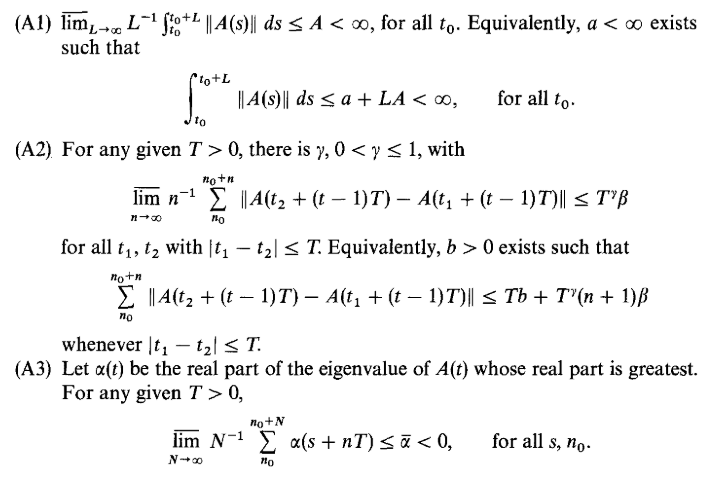
\includegraphics[width=0.7\linewidth]{Ref_4_Assumption_1_13.png}
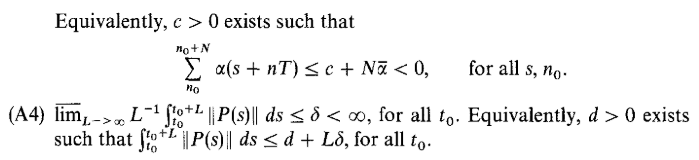
\includegraphics[width=0.68\linewidth]{Ref_4_Assumption_1_4.png}
\caption{Assumption A1-A4}
\end{figure}

This paper do not construct a Lyapunov function to prove stability, it directly goes to prove $|x(t)| \leq \beta |x(t_0)| e^{-\alpha (t-t_0)}$ by pick suitable parameters. These four assumptions are used for this theorem:
\begin{figure}[H]
\centering
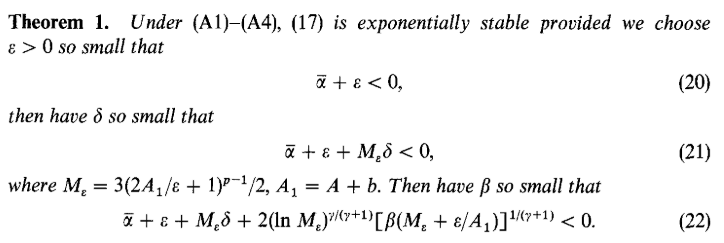
\includegraphics[width=0.7\linewidth]{Ref_4_Theorem_1.png}
\caption{Theorem 1}
\label{4_3A13}
\end{figure}

There are some discussion about the assumption (A2). The author showed us here, although (A2) is very similar to the differentiable condition, but it is weaker than differentiable. I think he want to give sufficient condition for his theorem to be true, so he gave up the strong assumption. However, in my point of view, since the system is slowly varying, $A$ won't change a lot in a short time, so differentiable assumption seems to be easy to achieve in practice, but I know it means totally different things in the mathematical proof.

The assumption (A3) is very similar to $\lim_{L \rightarrow \infty} L^{-1} \int_{t_0}^{t_0 + L} \alpha(u) du \leq \Bar{\alpha} < 0$ (3*), but they are not the same.  If we want to use (3*), we need to strengthen (2) to (2*): $||A(t+h)-A(t)|| \leq \beta h^{\gamma}$, for all $t$ and some $\gamma, 0<\gamma \leq 1$. Then we can generate a new theorem as follows:

\begin{figure}[H]
\centering
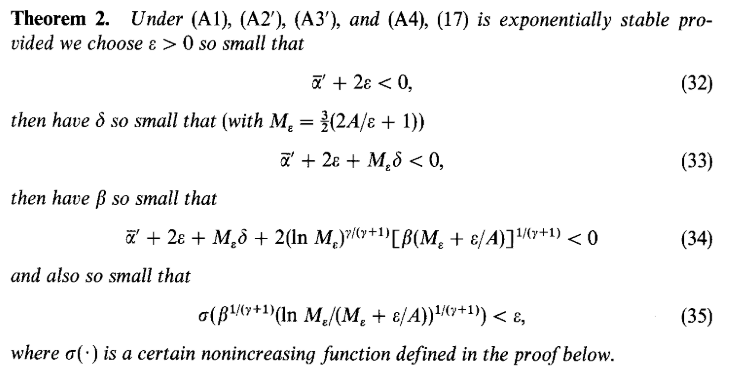
\includegraphics[width=0.7\linewidth]{Ref_4_Theorem_2.png}
\caption{Theorem 1}
\label{4_3A13}
\end{figure}

Until now, the majority work of this paper is done. We already talk about some details about the restrictions on $A$. Then the author continue apply the theorem to periodic situation and stochastic system. The proof method are very similar so I won't repeat it here. 

In summary, the most significant point in this paper is that the author relax one of the "standard" assumptions and proved the system still can achieve stability. 

\section{Part B}
$$\frac{d^2 y}{d t^2} = -\xi \frac{d y}{d t} + (a - 2 q cos(2t))y(t) \ (*)$$
$$\frac{d^2 y}{d t^2} + (-a + 2q \cdot cos(2t))y = 0 \ (**)$$
\subsection{Summary}
The differential equation $(*)$ is called Mathieu's Equation, with no damping term ($\xi = 0$) we can get (**). The lecture focus on the no-damping equation because it is easier to analyze. In the lecture, we use two variable extansion method to solve the stability question, it is a "reduced" method comes from Multiple Scales Method. But we need to notice here, this method works for small $q$ and it is not exactly precise while using just two variables. The system here is in the form:
$$\frac{d^2 x}{d t^2} + (\delta + \epsilon cos t)x = 0$$

By setting two variables ($t, \epsilon t$) with different scales, the system should hold for each of the scales, and these two variables will not effect each other. That is how the method works, we differentiate the equation so we change the original ODE to PDE. Then we extract the coefficients of the scale index $\epsilon^k$ $(k=0,1,2,...)$, which should be zero, and we get two equation for these two variables.
$$\frac{\partial^2 x_0}{\partial \xi^2} + \delta x_0 = 0$$
$$\frac{\partial^2 x_1}{\partial \xi^2} + \delta x_1 = - 2 \frac{\partial^2 x_0}{\partial \xi \partial \eta} - x_0 cos(\xi)$$

Then we can obtain the general solution for $x_0(\xi, \eta)$ and take it into the second equation. In the second equation we want to remove the resonance terms, so we will get: $$\frac{d A}{d \eta} = (\delta_1 - \frac{1}{2})B, \ \frac{d B}{d \eta} = - (\delta_1 + \frac{1}{2})A \Longrightarrow \frac{d^2 A}{d \eta^2} + (\delta_1^2 - \frac{1}{4})A = 0$$

So we can get the transition curves for the system 
$$\delta = \frac{1}{4} \pm \frac{\epsilon}{2} + O(\epsilon^2)$$

Besides this method, we have another two method to check the stability of Mathieu's Equation. The second method is to use Floquet theory on a generalization of Mathieu's Equation, we firstly change the Mathieu's Equation to:
$$\frac{d}{d t} \left[
  \begin{matrix}
  x_1 \\
  x_2
  \end{matrix}
  \right] = \left[
  \begin{matrix}
  0 & 1 \\
  -f(t) & 0
  \end{matrix}
  \right]\left[
  \begin{matrix}
  x_1 \\
  x_2
  \end{matrix}
  \right]$$
 
 then we construct a matrix $C$ which satisfies the specific initial conditions:
$$C = \left[\begin{matrix}
    x_{11}(t)&x_{21}(t)\\x_{12}(t)&x_{22}(t)
    \end{matrix}\right],  
    \left[\begin{matrix}
    x_{11}(0)&x_{21}(0)\\x_{12}(0)&x_{22}(0)
    \end{matrix}\right] =
    \left[\begin{matrix}
    1&0\\0&1
    \end{matrix}\right]$$

Then we calculate the eigenvalues of $C$: $\lambda = (trC \pm \sqrt{trC^2-4})$. From Floquet theory, the system will be stable if $|trC| < 2$. It seems to be most convenient method to solve this problem. However, we need to calculate $C$ numerically, which is very complex and difficult.\\
 
 The third method should be most suitable one, it is more precise than two variable expansion method and easier than Hill's Equation. It combined the first two methods to some extent. Using this method, we are aimed to find a solution in the form of a Fourier series, we can think it as infinity scales of method one, so the result should be more and more precise if we calculate more terms of the series. By constructing the determinant of coefficients matrix, we can easily take the first $k \times k$ matrix to get a approximated answer. If we want to get more precise anwer, the number $k$ can be larger. We use this method to solve the question in this part.
 
\subsection{Harmonic Balance}
The period of the the forcing function is $T = \pi$, so we can look for such a solution in the form of a Fourier series:
$$y(t) = \sum_{n=0}^{\infty} a_n cos(n t) + b_n sin(n t)$$
Thus, $$\frac{d y}{d t} = \sum_{n=0}^{\infty} - n \cdot a_n sin(n t) + n \cdot b_n cos(n t), \frac{d^2 y}{d t^2} = \sum_{n=0}^{\infty} - n^2 \cdot a_n cos(n t) - n^2 \cdot b_n sin(n t)$$
Therefore, 
$$(-a + 2q \cdot cos(2t)) y$$
$$= -a(\sum_{n=0}^{\infty} a_n cos(n t) + b_n sin(n t)) + 2q \cdot (\sum_{n=0}^{\infty} a_n \frac{1}{2} [cos((n+2) t) + cos((n-2)t)] + b_n \frac{1}{2} [sin((n+2) t)+sin((n-2)t))])$$
Take these into $(**)$, we can get the term with $a_0$ is $0 \cdot a_0 cos(0 t) - a \cdot a_0 \cdot cos(0 t) + 2q \cdot a_0 \cdot cos(2t) = -a \cdot a_0 + 2q \cdot a_0 \cdot cos(2t)$\\
the term with $a_2$ is $-4 a_2 cos(2t) - a \cdot a_2 cos(2t) + q \cdot a_2 (cos(4t) + cos(0 t)) = (-4-a) a_2 cos(2 t) + q \cdot a_2 cos(4t) + q \cdot a_2$\\
the term with $a_4$ is $-16 a_4 cos(4t) - a \cdot a_4 cos(4t) + q \cdot a_4 cos(6t) + q \cdot a_4 cos(2t)$\\
the term with $a_6$ is $-36 a_6 cos(6t) - a \cdot a_6 cos(6t) + q \cdot a_6 cos(8t) + q \cdot a_6 cos(4t)$\\
So the infinite determinant $a_{even}:$
$$\det{\begin{vmatrix} -a&q&0&0&...\\
2q&-a-4&q&0&...\\
0&q&-a-16&q&...\\
0&0&q&-a-36&...\\
& & ... & & \end{vmatrix}} = 0$$
The same for $b_{even}:$
$$\det{\begin{vmatrix} -a-4&q&0&0&...\\
q&-a-16&q&0&...\\
0&q&-a-36&q&...\\
0&0&q&-a-64&...\\
& & ... & & \end{vmatrix}} = 0$$
$a_{odd}:$
$$\det{\begin{vmatrix} -a-1+q&q&0&0&...\\
q&-a-9&q&0&...\\
0&q&-a-25&q&...\\
0&0&q&-a-49&...\\
& & ... & & \end{vmatrix}} = 0$$
$b_{odd}:$
$$\det{\begin{vmatrix} -a-1-q&q&0&0&...\\
q&-a-9&q&0&...\\
0&q&-a-25&q&...\\
0&0&q&-a-49&...\\
& & ... & & \end{vmatrix}} = 0$$
In all four determinants the typical row is of the form (except for the first one or two rows):
$$..., 0, q, -a-n^2, q, 0, ...$$
Following the notes, we can get the power series of $-a = n^2 + a_1 q + a_2 q^2 + ... \Longleftrightarrow a = -(n^2 + a_1 q + a_2 q^2 + ...)$. \\
Expanding a $3 \times 3$ truncation of the determinant, we get:
$$a_{even}: -a^3 - 20 a^2 + 2 a q^2 - 64*a + 16 q^2$$
$$b_{even}: -a^3 - 56 a^2 + 2 a q^2 - 784 a + 40 q^2 -2304$$
$$a_{odd}: -a^3 + a^2 q - 35 a^2 + 2 a q^2 + 34 a q - 259 q - q^3 + 26q^2 + 255 q -255$$
$$b_{odd}: -a^3 - a^2 q - 35 a^2 + 2 a q^2 -34 a q - 259 a + q^3 + 26 q^2 -255 q -255$$
Substituting the power series of $-a$ with $n = 0, 1, 2, ...$, we can get (compute by MatLab):
$$n=0, a_{even}: a = -(0-\frac{1}{2} q^2 + \frac{7}{128} q^4)$$
%$$n=0, b_{even}: a = -(0-\frac{5}{98} q^2 + \frac{15}{268912} q^4)$$
%$$n=0, a_{odd}: a = -(0-\frac{255}{259}q - \frac{39869}{354571} q^2 + \frac{1400204675}{166494840757} q^3 + \frac{316455314088}{1595520058974331} q^4 - \frac{16039201600944331}{107029081076057097811} q^5)$$
%$$n=0, b_{odd}: a = -(0 + \frac{255}{259}q - \frac{39869}{354571} q^2 - \frac{1400204675}{166494840757} q^3 + \frac{316455314088}{1595520058974331} q^4 + \frac{16039201600944331}{107029081076057097811} q^5)$$
%$$n=1, a_{even}: a = -(1-\frac{29}{27} q^2 + \frac{11948}{19683} q^4)$$
%$$n=1, b_{even}: a = -(1-\frac{38}{675} q^2 - \frac{25232}{307546875} q^4)$$
$$n=1, a_{odd}: a = -(1-q - \frac{1}{8} q^2 + \frac{1}{64} q^3 - \frac{1}{1536}q^4 - \frac{11}{36864}q^5)$$
$$n=1, b_{odd}: a = -(1+q - \frac{1}{8} q^2 - \frac{1}{64} q^3 - \frac{1}{1536}q^4 + \frac{11}{36864}q^5)$$
$$n=2, a_{even}: a = -(4+\frac{5}{12} q^2 - \frac{95}{1728} q^4)$$
$$n=2, b_{even}: a = -(4-\frac{1}{12} q^2 + \frac{5}{13824} q^4)$$
%$$n=2, a_{odd}: a = -(4-\frac{35}{9}q + \frac{18527}{2187} q^2 - \frac{24766609}{531441} q^3 + \frac{40531437544}{129140163}q^4 - \frac{74060841539185}{31381059609}q^5)$$
%$$n=2, b_{odd}: a = -(4+\frac{35}{9}q + \frac{18527}{2187} q^2 + \frac{24766609}{531441} q^3 + \frac{40531437544}{129140163}q^4 + \frac{74060841539185}{31381059609}q^5)$$
Therefore, we can draw a picture as follows:
\begin{figure}[h!]
\centering
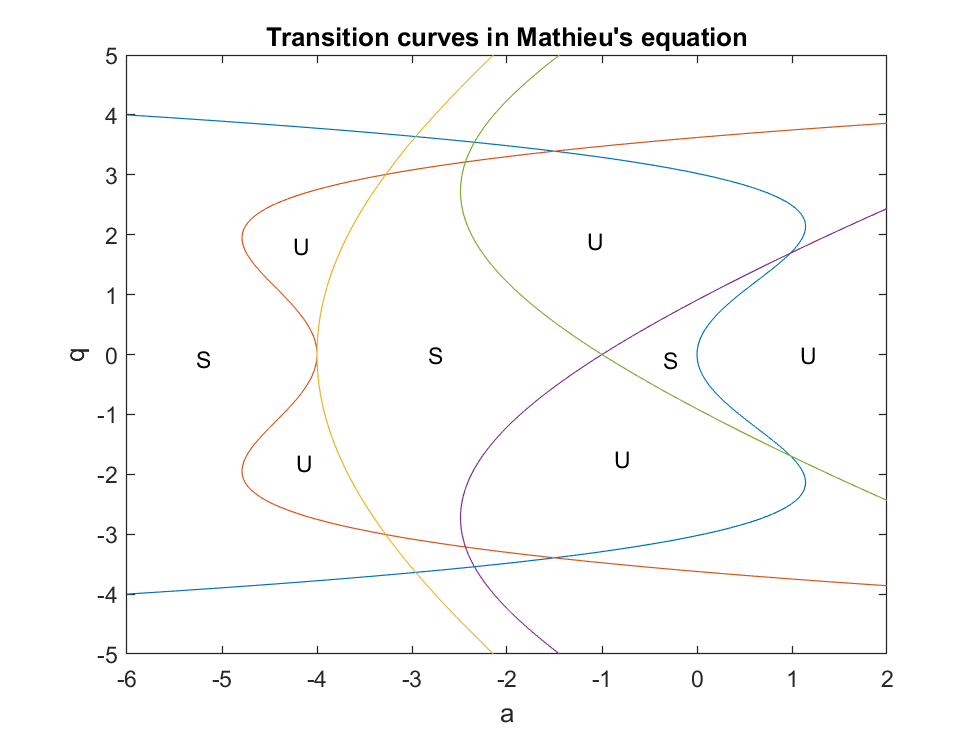
\includegraphics[width=0.6\linewidth]{Part_B_Result.png}
\end{figure}

All the MatLab code for Part B.B is attached in the end of this report.

\subsection{With Damping Term}
If we introduce damping, we still can use two variable expansion method to analyze the system (Here we assume $q$ is small). We can follow the same way as notes do. Notice here, in our equation, $-a = \delta$ and $2q = \epsilon$, so for $n = 1$, the transition curves will change to 
$$a = -(1 \pm \sqrt{1-\mu^2}q + O(q^2))$$

Compare to the result we get from B:
$$a = -(1 \pm q - \frac{1}{8} q^2 + \frac{1}{64} q^3 - \frac{1}{1536}q^4 - \frac{11}{36864}q^5)$$

We can easily conclude that, \textbf{for introducing the damping term, the original stable condition will still hold, and some of the original unstable part will turn to stable}.

Here we can consider this problem in another way. We consider something related to "Energy". When the system add a damping term, it means the "Energy" of the system will decrease, so it should be more stable than without damping. Therefore, without Mathematical proof, it is intuitive for me to claim the system will be more stable. 

\section{Part C (Option C.1)}
$$\dot{x}(t) =  \left[
 \begin{matrix}
   0 & 1 & 0 & 0 \\
   3\omega_0^2 & 0 & 0 & 2\omega_0 \\
   0 & 0 & 0 & 1 \\
   0 & -2\omega_0 & 0 & 0
  \end{matrix}
  \right] x(t) + \left[
  \begin{matrix}
  0 & 0 \\
  1 & 0 \\
  0 & 0 \\
  0 & 1
  \end{matrix}
  \right] u(t) = A x + B u$$
 $$y = [x_1, x_3]^T = \left[
  \begin{matrix}
  1 & 0 & 0 & 0\\
  0 & 0 & 1 & 0
  \end{matrix}
  \right] \left[
  \begin{matrix}
  x_1 \\
  x_2 \\
  x_3 \\
  x_4
  \end{matrix}
  \right] = C x \ (D = 0)$$
\subsection{a}
For this LTI system, the state-transition matrix (by MatLab) $\Phi_A(t,\tau) = e^{A(t-\tau)} = \mathcal{L}^{-1}\{[s I-A]^{-1}\} = $
$$\left[
 \begin{matrix}
   4-3 cos(\omega_0 (t-\tau)) & sin(\omega_0 (t-\tau)) / \omega_0 & 0 & 2/\omega_0 - 2 cos(\omega_0 (t-\tau))/ \omega_0 \\
   3\omega_0 sin(\omega_0 (t-\tau)) & cos(\omega_0 (t-\tau)) & 0 & 2 sin(\omega_0 (t-\tau)) \\
   6sin(\omega_0(t - \tau)) - 6\omega_0(t-\tau) & (2cos(\omega_0(t - \tau)) - 2)/\omega_0& 1& (4sin(\omega_0(t - \tau)) - 3 \omega_0 (t-\tau))/\omega_0\\
    6\omega_0(cos(\omega_0(t - \tau)) - 1)& -2sin(\omega_0(t - \tau))& 0&4cos(\omega_0(t - \tau)) - 3
  \end{matrix}
  \right]$$
For the impulse response matrix $y(t) = C \Phi_A (t,\tau) B =$
$$\left[
  \begin{matrix}
  sin(\omega_0 (t-\tau))/\omega_0 & 2/\omega_0 - 2 cos(\omega_0 (t-\tau))/\omega_0 \\
  2 cos(\omega_0 (t-\tau))/\omega_0 - 2/\omega_0 & 4 sin(\omega_0 (t-\tau))/\omega_0 - 3(t-\tau)
  \end{matrix}
  \right]$$
and transfer function matrix $G(s) = C (s I - A)^{-1} B =$ $$\left[
  \begin{matrix}
  \frac{1}{s^2 + \omega_0^2} & \frac{2\omega_0}{s^3+s\omega_0^2} \\
  -\frac{2\omega_0}{s^3 + s\omega_0^2}& \frac{s^2 - 3\omega_0^2}{s^4 + s^2\omega_0^2}
  \end{matrix}
  \right]$$
\subsection{b}
Here the sampling time is $t_s$, so $A_d = e^{A T} = e^{A t_s} =$
$$\left[
 \begin{matrix}
   4-3 cos(\omega_0 t_s) & sin(\omega_0 t_s) / \omega_0 & 0 & 2/\omega_0 - 2 cos(\omega_0 t_s)/ \omega_0 \\
   3\omega_0 sin(\omega_0 t_s) & cos(\omega_0 t_s) & 0 & 2 sin(\omega_0 t_s) \\
   6sin(\omega_0 t_s) - 6\omega_0 t_s & (2cos(\omega_0 t_s) - 2)/\omega_0& 1& (4sin(\omega_0 t_s) - 3 \omega_0 t_s)/\omega_0\\
    6\omega_0(cos(\omega_0 t_s) - 1)& -2sin(\omega_0 t_s)& 0&4cos(\omega_0 t_s) - 3
  \end{matrix}
  \right]$$
and $B_d = [\int_0^T e^{A \sigma} d \sigma] B =$
$$\left[
 \begin{matrix}
   2 sin(t_s \omega_0/2)^2 / \omega_0^2 & - 2(sin(t_s \omega_0)-t_s \omega_0)/ \omega_0^2 \\
   sin(t_s \omega_0)/ \omega_0 & 4 sin(t_s \omega_0)^2 / \omega_0 \\
   (2(sin(t_s \omega_0) - t_s \omega_0))/\omega_0^2 & (8sin((t_s \omega_0)/2)^2)/\omega_0^2 - (3t_s^2)/2\\
  -(4sin((t_s \omega_0)/2)^2)/\omega_0 & (4sin(t_s \omega_0))/\omega_0 - 3t_s
  \end{matrix}
  \right]$$
$x[k+1] = A_d x[k] \rightarrow x[k] = A_d^{k-l} x[l], k \ge l$, so the discrete-time state-transition matrix is $\phi_A(k,l) = A_d^{k-l}$, so:
$$\Phi_{A_d}(k,l) = \left[
 \begin{matrix}
   4-3 cos(\omega_0 (k - l) t_s) & sin(\omega_0 (k - l) t_s) / \omega_0 & 0 & 2/\omega_0 - 2 cos(\omega_0 (k - l) t_s)/ \omega_0 \\
   3\omega_0 sin(\omega_0 (k - l) t_s) & cos(\omega_0 (k - l) t_s) & 0 & 2 sin(\omega_0 (k - l) t_s) \\
   6sin(\omega_0 (k - l) t_s) - 6\omega_0 (k - l) t_s & (2cos(\omega_0 (k - l) t_s) - 2)/\omega_0& 1& (4sin(\omega_0 (k - l) t_s) - 3 \omega_0 (k - l) t_s)/\omega_0\\
    6\omega_0(cos(\omega_0 (k - l) t_s) - 1)& -2sin(\omega_0 (k - l) t_s)& 0&4cos(\omega_0 (k - l) t_s) - 3
  \end{matrix}
  \right]$$
where $t_s = 0.01$ \\
The eigenvalues of $A_d$ are: $\lambda_1 = 1,\lambda_2 = 1,\lambda_3 = cos(0.01 \omega_0) - sin(0.01 \omega_0) i, \lambda_4 = cos(0.01 \omega_0) + sin(0.01 \omega_0)i$, so two ($\lambda_1$ and $\lambda_2$) of eigenvalues of $A_d$ are on the $1$ and the other two ($\lambda_4$ and $\lambda_4$) are on the circle which centered in the origin, radius = $1$, and these two eigenvalues are conjugate.
\subsection{c}
For this LTI system, 
$$\Delta(\lambda) = \det (\lambda I - A) = \lambda^4 + \omega_0^2 \lambda^2 = \lambda^2 (\lambda^2 + \omega_0^2) = 0$$

so the eigenvalue of $A$ are $\lambda_k = 0, 0, \omega_0 i, -\omega_0 i$ $(k = 1,2,3,4)$, and $Re (\lambda_k) = 0$, so the system is not UES.

$\Psi(\lambda) = \lambda^2 (\lambda^2 + \omega_0^2) = 0 \rightarrow$ It is also not US because the eigenvalue $\lambda_{1,2} = 0$ are not simple.

From the transfer function, we can get the poles: 
$$\left[
 \begin{matrix}
   (\omega_0 i, - \omega_0 i) & (0, \omega_0 i, - \omega_0 i) \\
   (0, \omega_0 i, - \omega_0 i) & (0,0, \omega_0 i, - \omega_0 i)
  \end{matrix}
  \right]$$

Since there is a zero pole, so it is not BIBO stable.
\subsection{d}
For this LTI system, we can check $rank(Q_c)$ and $rank(Q_o)$ for the Controllability and Observability.
$$rank(Q_c) = rank(B | AB | A^2 B | A^3 B) = 4$$
$$rank(Q_o) = rank(\left[
 \begin{matrix}
    C \\
    CA \\
    CA^2 \\
    CA^3
  \end{matrix}
  \right]) = 4$$
  
They are all full rank matrices, so this system is observable and controllable.

Controllability gramian matrix $W(t_0, t_f) = \int_{t_0}^{t_f} \Phi_A(t_0, \sigma) B(\sigma)B^T(\sigma) \Phi_A^T (t_0, \sigma)d \sigma = \int_{t_0}^{t_f} e^{A(t_0- \sigma)} B B^T e^{A^T(t_0- \sigma)} d \sigma$ 
$$W(:, 1) = \left(\begin{array}{c} -\frac{\frac{3\,\sin\left(2\,w\,\left(t_{0}-\mathrm{tf}\right)\right)}{4}-8\,\sin\left(w\,\left(t_{0}-\mathrm{tf}\right)\right)+w\,\left(\frac{13\,t_{0}}{2}-\frac{13\,\mathrm{tf}}{2}\right)}{w^3}\\ \frac{3\,{\sin\left(w\,\left(t_{0}-\mathrm{tf}\right)\right)}^2-16\,{\sin\left(\frac{w\,\left(t_{0}-\mathrm{tf}\right)}{2}\right)}^2}{2\,w^2}\\ \frac{3\,{\left(\sin\left(w\,\left(t_{0}-\mathrm{tf}\right)\right)-t_{0}\,w+\mathrm{tf}\,w\right)}^2}{w^3}\\ \frac{\frac{3\,\sin\left(2\,w\,\left(t_{0}-\mathrm{tf}\right)\right)}{2}-14\,\sin\left(w\,\left(t_{0}-\mathrm{tf}\right)\right)+w\,\left(11\,t_{0}-11\,\mathrm{tf}\right)}{w^2} \end{array}\right)$$
$$W(:, 2) = \left(\begin{array}{c} \frac{3\,{\sin\left(w\,\left(t_{0}-\mathrm{tf}\right)\right)}^2-16\,{\sin\left(\frac{w\,\left(t_{0}-\mathrm{tf}\right)}{2}\right)}^2}{2\,w^2}\\ \frac{5\,\mathrm{tf}}{2}-\frac{5\,t_{0}}{2}+\frac{3\,\sin\left(2\,w\,\left(t_{0}-\mathrm{tf}\right)\right)}{4\,w}\\ \frac{16\,\sin\left(w\,\left(t_{0}-\mathrm{tf}\right)\right)+3\,\sin\left(2\,w\,\left(t_{0}-\mathrm{tf}\right)\right)-10\,t_{0}\,w+10\,\mathrm{tf}\,w-12\,t_{0}\,w\,\cos\left(w\,\left(t_{0}-\mathrm{tf}\right)\right)+12\,\mathrm{tf}\,w\,\cos\left(w\,\left(t_{0}-\mathrm{tf}\right)\right)}{2\,w^2}\\ -\frac{3\,\left({\sin\left(w\,\left(t_{0}-\mathrm{tf}\right)\right)}^2-4\,{\sin\left(\frac{w\,\left(t_{0}-\mathrm{tf}\right)}{2}\right)}^2\right)}{w} \end{array}\right)$$

$W(:,3) = $

$$\left(\begin{array}{c} \frac{3\,{\left(\sin\left(w\,\left(t_{0}-\mathrm{tf}\right)\right)-t_{0}\,w+\mathrm{tf}\,w\right)}^2}{w^3}\\ \frac{16\,\sin\left(w\,\left(t_{0}-\mathrm{tf}\right)\right)+3\,\sin\left(2\,w\,\left(t_{0}-\mathrm{tf}\right)\right)-10\,t_{0}\,w+10\,\mathrm{tf}\,w-12\,t_{0}\,w\,\cos\left(w\,\left(t_{0}-\mathrm{tf}\right)\right)+12\,\mathrm{tf}\,w\,\cos\left(w\,\left(t_{0}-\mathrm{tf}\right)\right)}{2\,w^2}\\ \frac{32\,\sin\left(w\,\left(t_{0}-\mathrm{tf}\right)\right)+3\,\sin\left(2\,w\,\left(t_{0}-\mathrm{tf}\right)\right)-3\,{t_{0}}^3\,w^3+3\,{\mathrm{tf}}^3\,w^3-14\,t_{0}\,w+14\,\mathrm{tf}\,w-24\,t_{0}\,w\,\cos\left(w\,\left(t_{0}-\mathrm{tf}\right)\right)+24\,\mathrm{tf}\,w\,\cos\left(w\,\left(t_{0}-\mathrm{tf}\right)\right)-9\,t_{0}\,{\mathrm{tf}}^2\,w^3+9\,{t_{0}}^2\,\mathrm{tf}\,w^3}{w^3}\\ 9\,t_{0}\,\mathrm{tf}-\frac{6\,{\sin\left(w\,\left(t_{0}-\mathrm{tf}\right)\right)}^2}{w^2}-\frac{8\,{\sin\left(\frac{w\,\left(t_{0}-\mathrm{tf}\right)}{2}\right)}^2}{w^2}-\frac{9\,{t_{0}}^2}{2}-\frac{9\,{\mathrm{tf}}^2}{2}+\frac{12\,t_{0}\,\sin\left(w\,\left(t_{0}-\mathrm{tf}\right)\right)}{w}-\frac{12\,\mathrm{tf}\,\sin\left(w\,\left(t_{0}-\mathrm{tf}\right)\right)}{w} \end{array}\right)$$

$$W(:,4) = \left(\begin{array}{c} \frac{\frac{3\,\sin\left(2\,w\,\left(t_{0}-\mathrm{tf}\right)\right)}{2}-14\,\sin\left(w\,\left(t_{0}-\mathrm{tf}\right)\right)+w\,\left(11\,t_{0}-11\,\mathrm{tf}\right)}{w^2}\\ -\frac{3\,\left({\sin\left(w\,\left(t_{0}-\mathrm{tf}\right)\right)}^2-4\,{\sin\left(\frac{w\,\left(t_{0}-\mathrm{tf}\right)}{2}\right)}^2\right)}{w}\\ 9\,t_{0}\,\mathrm{tf}-\frac{6\,{\sin\left(w\,\left(t_{0}-\mathrm{tf}\right)\right)}^2}{w^2}-\frac{8\,{\sin\left(\frac{w\,\left(t_{0}-\mathrm{tf}\right)}{2}\right)}^2}{w^2}-\frac{9\,{t_{0}}^2}{2}-\frac{9\,{\mathrm{tf}}^2}{2}+\frac{12\,t_{0}\,\sin\left(w\,\left(t_{0}-\mathrm{tf}\right)\right)}{w}-\frac{12\,\mathrm{tf}\,\sin\left(w\,\left(t_{0}-\mathrm{tf}\right)\right)}{w}\\ 19\,\mathrm{tf}-19\,t_{0}+\frac{24\,\sin\left(w\,\left(t_{0}-\mathrm{tf}\right)\right)-3\,\sin\left(2\,w\,\left(t_{0}-\mathrm{tf}\right)\right)}{w} \end{array}\right)$$

\subsection{e}
From the notes, $u(t) = B^T \Phi_A^T(t_0, t) W^{-1}(t_0, t_f) [\Phi_A(t_0, t_f) x_f - x_0]$, where $x_0 = [0,0,\theta,0]^T, x(t_f) = [0,0,(\omega_0 t_f - \theta),0]^T$

$u(t)$ is too long to print out in one page, \textbf{please check my MatLab code for this question}.

From this $u(t)$, we can simulate the closed-loop system numerically. The following pictures are the results. Since $t_f \in [0.1, 2]$,  I select $t_f = 0.1$,$1$ and $2$ for the simulation, the pictures on the left with $\theta = \pi/10$ and the pictures on the right with $\theta = -\pi/10$

\begin{figure}[H]
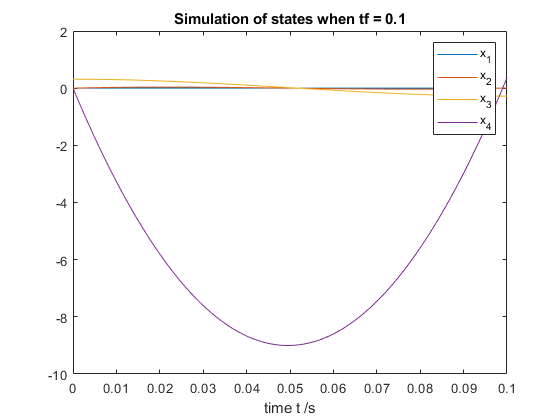
\includegraphics[width=0.5\linewidth]{simulation_tf_01.png}
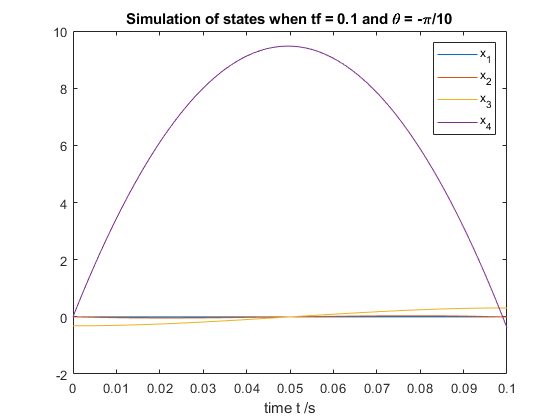
\includegraphics[width=0.5\linewidth]{simulation_tf_01_m.png}
\end{figure}

\begin{figure}[H]
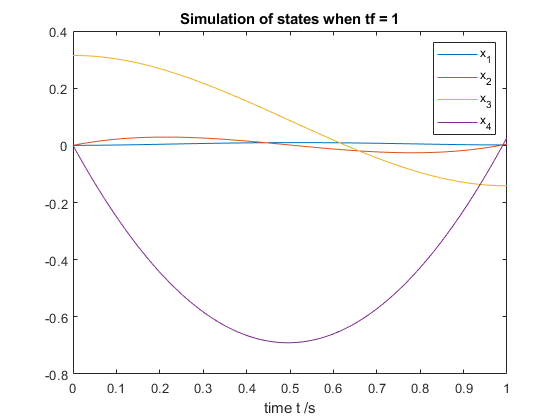
\includegraphics[width=0.5\linewidth]{simulation_tf_1.png}
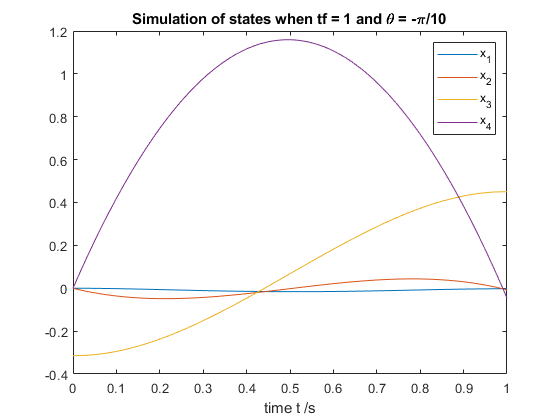
\includegraphics[width=0.5\linewidth]{simulation_tf_1_m.png}
\end{figure}

\begin{figure}[H]
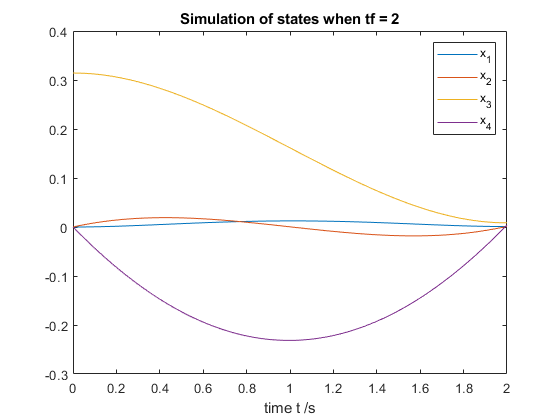
\includegraphics[width=0.5\linewidth]{simulation_tf_2.png}
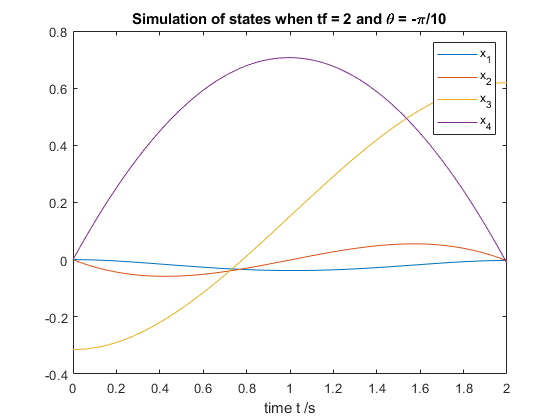
\includegraphics[width=0.5\linewidth]{simulation_tf_2_m.png}
\end{figure}

The result will change if we change the value of $\theta$ to $-\pi/10$. It is a LTI system, if the system vary from the opposite initial state to opposite final state, it should be sign reversal. However the final state is not reversal completely, it has a bias term $\omega_0 t_f$, so the picture are not reversal although it looks like so. 

For the same reason, the energy shouldn't be the same. By changing the value of $t_f$, we can get different total energy consumption $J$, the following picture shows when $t_f$ varys from $0.01$ to $2$, how the $J$ changes. The red line is for $\theta = \pi/10$ and the blue line is for $\theta = - \pi/10$.

\begin{figure}[H]
\centering
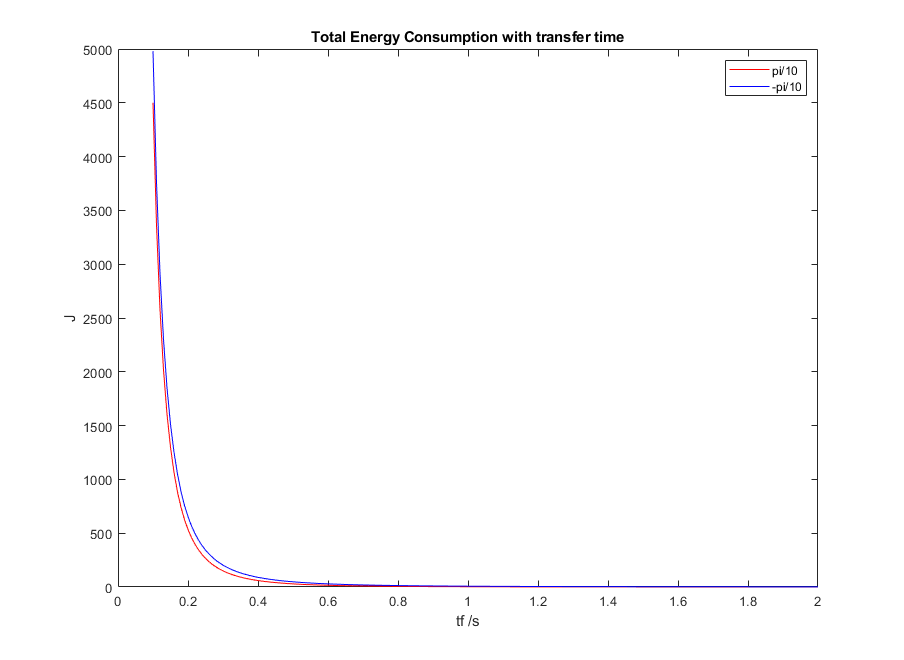
\includegraphics[width=0.6\linewidth]{Part_C_e_1.png}
\caption{Total Energy Consumption Graph}
\end{figure}

\begin{figure}[H]
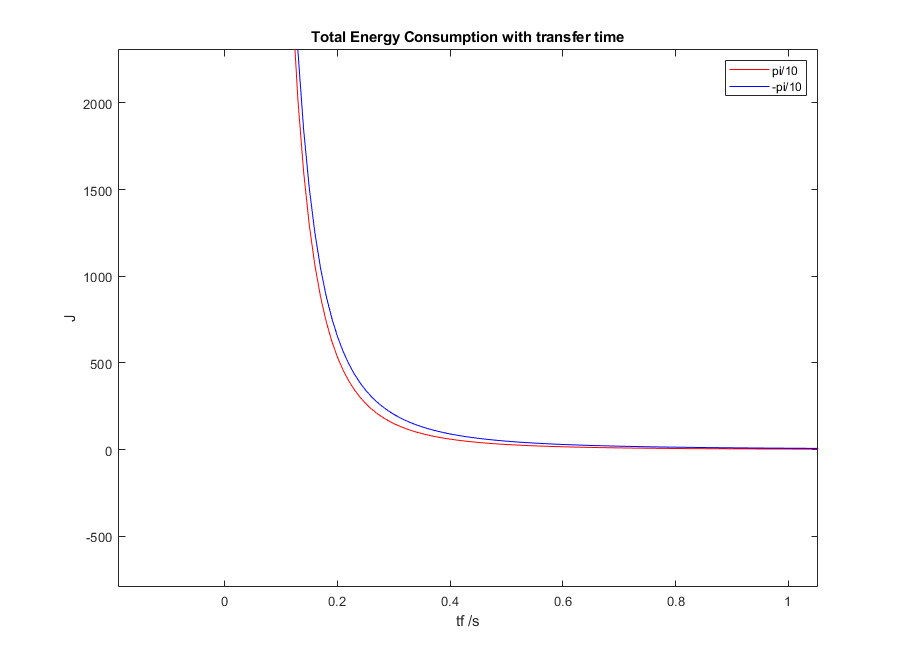
\includegraphics[width=0.5\linewidth]{Part_C_e_2.png}
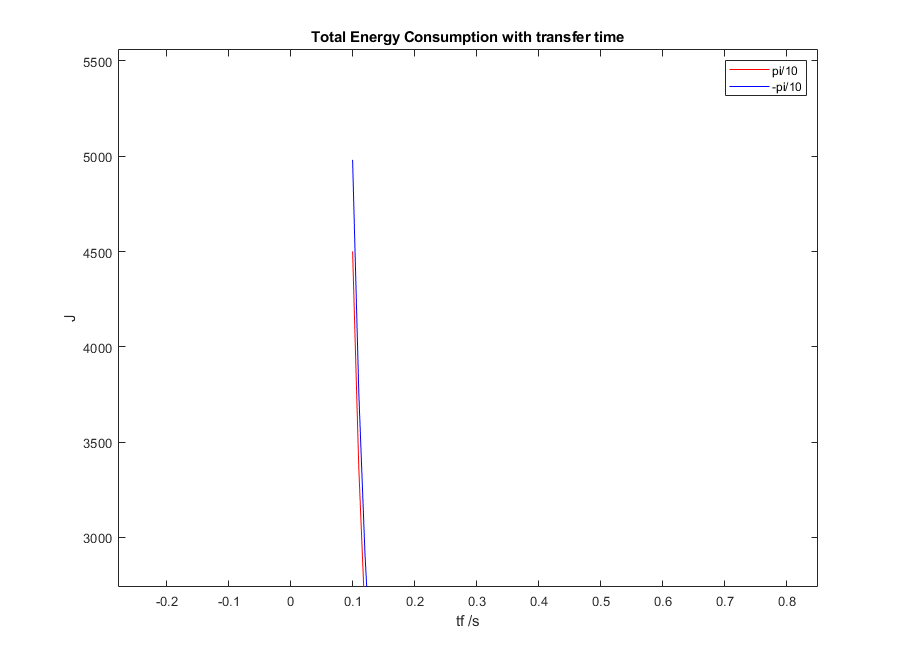
\includegraphics[width=0.5\linewidth]{Part_C_e_3.png}
\caption{Details of Energy Graph}
\end{figure}

\subsection{f}
Let set the observer $\hat{\dot{x}}(t) = A \hat{x} + B u + L(y - C \hat{x}) = (A - LC)\hat{x} + B u + L y$, so the new $A$ matrix is $\hat{A} = A - LC$. Then we calculate the eigenvalue of $\hat{A}$:
$$\det (\lambda I - \hat{A}) = {\begin{vmatrix} 
\lambda + L_{11}& -1 & L_{12} & 0 \\
L_{21} - 3 \omega_0^2& \lambda & L_{22} & -2 \omega_0\\
L_{31} & 0 &\lambda + L_{32} & -1\\
L_{41} & 2 \omega_0 & L_{42} & \lambda
\end{vmatrix}}$$
$$= \lambda^4 + (L_{11} + L_{32})\lambda^3 + (\omega_0^2 + L_{21} + L_{42} + L_{11}L_{32})\lambda^2$$ 
$$+ (2 L_{41} \omega_0 - 2 L_{22} \omega_0 + 4 L_{11} \omega_0^2 + L_{11}L_{42} - L_{12} L_{41} + L_{21} L_{32} - L_{22} L_{31})\lambda + L_{21}*L_{42} - 3 L_{42} \omega_0^2 - 6 L_{12} \omega_0^3$$
$$- L_{22} L_{41}-2 L_{11} L_{22} \omega + 2 L_{12} L_{21} \omega_0 - 2 L_{31} L_{42} \omega_0 + 2 L_{32} L_{41} \omega_0 + 4 L_{11} L_{32} \omega_0^2 - 4*L_{12} L_{31} \omega_0^2$$
It should be same as $(\lambda + 0.5)(\lambda + 2.5)(\lambda + 0.5 + j)(\lambda + 0.5 - j)$
$$= \lambda^4 + 4 \lambda^3 + \frac{11}{2} \lambda^2 + 5 \lambda + \frac{25}{16}$$
Which means:
$$L_{11} + L_{32} = 4$$
$$\omega_0^2 + L_{21} + L_{42} + L_{11}L_{32} = \frac{11}{2}$$
$$2 L_{41} \omega_0 - 2 L_{22} \omega_0 + 4 L_{11} \omega_0^2 + L_{11}L_{42} - L_{12} L_{41} + L_{21} L_{32} - L_{22} L_{31} = 5$$
$$L_{21}*L_{42} - 3 L_{42} \omega_0^2 - 6 L_{12} \omega_0^3 - L_{22} L_{41}-2 L_{11} L_{22} \omega + 2 L_{12} L_{21} \omega_0 - 2 L_{31} L_{42} \omega_0 + 2 L_{32} L_{41} \omega_0 + 4 L_{11} L_{32} \omega_0^2 - 4*L_{12} L_{31} \omega_0^2=\frac{25}{16}$$

Using MatLab I cannot solve this equation, so I change to use another method. If the observer exist, the Sylvester equation $T A + F T = \hat{L} C$ must have a non-singular solution $T$ and $L = (T^{-1})^T \hat{L}$. $F$ has the same eigenvalues as $\hat{A}$,let
$$F = \left[
 \begin{matrix}
    -0.5 & 0 & 0 & 0 \\
    0 & -2.5 & 0 & 0 \\
    0 & 0 & -0.5+j & 0 \\
    0 & 0 & 0& -0.5-j
  \end{matrix}
  \right], \hat{L} = \left[
 \begin{matrix}
    1 & 1& 1& 1\\
    1&1&1&1
  \end{matrix}
  \right]$$
  
Using MatLab we can get:
$$L = \left(\begin{array}{cc} -\frac{-24\,w^4-48\,w^3+132\,w^2+60\,w+25}{60\,w^3} & -\frac{-24\,w^4-48\,w^3+132\,w^2+60\,w+25}{60\,w^3}\\ -\frac{16\,w^4-128\,w^3-88\,w^2+160\,w+25}{80\,w^2} & -\frac{16\,w^4-128\,w^3-88\,w^2+160\,w+25}{80\,w^2}\\ \frac{-24\,w^4+192\,w^3+132\,w^2+60\,w+25}{60\,w^3} & \frac{-24\,w^4+192\,w^3+132\,w^2+60\,w+25}{60\,w^3}\\ \frac{-64\,w^4-128\,w^3+352\,w^2+160\,w+25}{80\,w^2} & \frac{-64\,w^4-128\,w^3+352\,w^2+160\,w+25}{80\,w^2} \end{array}\right)$$

Check the eigenvalue of $\hat{A}=A-LC$, it satisfies the requirement.

\begin{figure}[H]
\centering
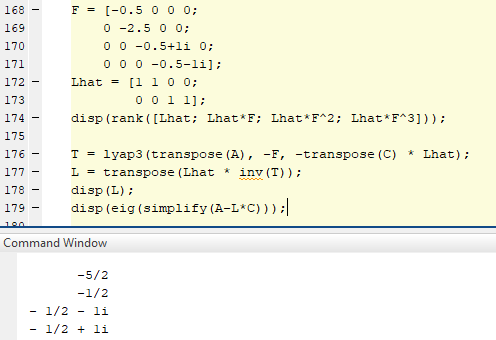
\includegraphics[width=0.5\linewidth]{Part_C_f.png}
\caption{MatLab Result for checking eigenvalue}
\end{figure}

\subsection{g}
From \cite{engel2002continuous}, we need to construct the matrix $H$ with a given $D$, to make $F$ stable and $\det [T, e^{FD}T] \neq 0$. Therefore the system:
$$\dot{z} = F z + H y + G u, t \ge t_0$$
$$\hat{x}(t) = K[z(t)-e^{FD} z(t-D)], K := [I_{n,n}, 0_{n,n}][T, e^{FD}T]^{-1}$$

the state estimate $\hat{x}$ will converges to x in finite time $D$. And here:
$$F_i := A - H_i C, i=1,2$$
$$F := \left[
 \begin{matrix}
    F_1 & 0 \\
    0 & F_2
  \end{matrix}
  \right], H := \left[
 \begin{matrix}
    H_1 \\
    H_2
  \end{matrix}
  \right], G := \left[
 \begin{matrix}
    B \\
    B
  \end{matrix}
  \right], T := \left[
 \begin{matrix}
    I_{n,n} \\
    I_{n,n}
  \end{matrix}
  \right], z := \left[
 \begin{matrix}
    z_1 \\
    z_2
  \end{matrix}
  \right]$$

And from the Lemma in the \cite{engel2002continuous}, it should be easier if we make $Re \lambda_j (F_2) < \sigma < Re \lambda_j (F_1), j = 1,2,3,...,n$

Therefore, we can choose the eigenvalues of $F_1$ to be $\{-1,-2,-3,-4\}$ and eigenvalues of $F_2$ to be $\{-7,-8,-9,-10\}$, then we can use the same method from Part C.$f$ to get $H$. After this, check whether $\det [T, e^{FD}T] \neq 0$, if it is true. we are done.

Using MatLab, we can get 
$$H_1 = \left(\begin{array}{cc} -\frac{2\,\left(-w^4-5\,w^3+35\,w^2+25\,w+16\right)}{5\,w^3} & -\frac{2\,\left(-w^4-5\,w^3+35\,w^2+25\,w+16\right)}{5\,w^3}\\ -\frac{w^4-20\,w^3-35\,w^2+100\,w+24}{5\,w^2} & -\frac{w^4-20\,w^3-35\,w^2+100\,w+24}{5\,w^2}\\ \frac{2\,\left(-w^4+20\,w^3+35\,w^2+25\,w+16\right)}{5\,w^3} & \frac{2\,\left(-w^4+20\,w^3+35\,w^2+25\,w+16\right)}{5\,w^3}\\ \frac{4\,\left(-w^4-5\,w^3+35\,w^2+25\,w+6\right)}{5\,w^2} & \frac{4\,\left(-w^4-5\,w^3+35\,w^2+25\,w+6\right)}{5\,w^2} \end{array}\right)$$

$$H_2 = \left(\begin{array}{cc} -\frac{2\,\left(-w^4-17\,w^3+431\,w^2+1207\,w+3360\right)}{5\,w^3} & -\frac{2\,\left(-w^4-17\,w^3+431\,w^2+1207\,w+3360\right)}{5\,w^3}\\ -\frac{w^4-68\,w^3-431\,w^2+4828\,w+5040}{5\,w^2} & -\frac{w^4-68\,w^3-431\,w^2+4828\,w+5040}{5\,w^2}\\ \frac{2\,\left(-w^4+68\,w^3+431\,w^2+1207\,w+3360\right)}{5\,w^3} & \frac{2\,\left(-w^4+68\,w^3+431\,w^2+1207\,w+3360\right)}{5\,w^3}\\ \frac{4\,\left(-w^4-17\,w^3+431\,w^2+1207\,w+1260\right)}{5\,w^2} & \frac{4\,\left(-w^4-17\,w^3+431\,w^2+1207\,w+1260\right)}{5\,w^2} \end{array}\right)$$

And $\det [T, e^{FD}T] \neq 0$, which means we are done!

\bibliographystyle{plain}
\bibliography{reference}

\newpage
\section{Appendix: MatLab Code}
\begin{lstlisting}
%% This is for Part B
N = 3;
Ae = zeros(N,5);
Be = zeros(N,5);
Ao = zeros(N,5);
Bo = zeros(N,5);

for n = 0:1:N-1
    P = 3;
    syms a q a1 a2 a3 a4 a5;
    a = -(n^2 + a1*q + a2*q^2 + a3*q^3 + a4*q^4 + a5*q^5);
    Aeven = sym(zeros(P));
    Beven = sym(zeros(P));
    Aodd = sym(zeros(P));
    Bodd = sym(zeros(P));
    Aeven(1, 1:2) = [-a, q];
    Beven(1, 1:2) = [-a-4, q];
    Aodd(1, 1:2) = [-a-1+q, q];
    Bodd(1, 1:2) = [-a-1-q, q];
    for i = 2:1:P-1
        if i == 2
            Aeven(i, i-1:i+1) = [2*q, -a-(2*i-2)^2, q];
        else
            Aeven(i, i-1:i+1) = [q, -a-(2*i-2)^2, q];
        end
        Beven(i, i-1:i+1) = [q, -a-(2*i)^2, q];
        Aodd(i, i-1:i+1) = [q, -a-(2*i-1)^2, q];
        Bodd(i, i-1:i+1) = [q, -a-(2*i-1)^2, q];
    end
    Aeven(P, P-1:P) = [q, -a-(2*P-2)^2];
    Beven(P, P-1:P) = [q, -a-(2*P)^2];
    Aodd(P, P-1:P) = [q, -a-(2*P-1)^2];
    Bodd(P, P-1:P) = [q, -a-(2*P-1)^2];

    detAeven = det(Aeven);
    disp(detAeven);
    detBeven = det(Beven);
    disp(detBeven);
    detAodd = det(Aodd);
    disp(detAodd);
    detBodd = det(Bodd);
    disp(detBodd);
    
    [c,~]= poly_coeffs(detAeven,'q');
    [ae10,ae20,ae30,ae40,ae50] = solve(c(end-5),c(end-4),c(end-3),c(end-2),...
        c(end-1),a1,a2,a3,a4,a5);
    Ae(n+1, 1) = ae10;
    Ae(n+1, 2) = ae20;
    Ae(n+1, 3) = ae30;
    Ae(n+1, 4) = ae40;
    Ae(n+1, 5) = ae50;
    
    [c,~]= poly_coeffs(detBeven,'q');
    [be10,be20,be30,be40,be50] = solve(c(end-5),c(end-4),c(end-3),c(end-2),...
        c(end-1),a1,a2,a3,a4,a5);
    Be(n+1, 1) = be10;
    Be(n+1, 2) = be20;
    Be(n+1, 3) = be30;
    Be(n+1, 4) = be40;
    Be(n+1, 5) = be50;
    
    [c,~]= poly_coeffs(detAodd,'q');
    [ao10,ao20,ao30,ao40,ao50] = solve(c(end-5),c(end-4),c(end-3),c(end-2),...
        c(end-1),a1,a2,a3,a4,a5);
    Ao(n+1, 1) = ao10;
    Ao(n+1, 2) = ao20;
    Ao(n+1, 3) = ao30;
    Ao(n+1, 4) = ao40;
    Ao(n+1, 5) = ao50;
    
    [c,~]= poly_coeffs(detBodd,'q');
    [bo10,bo20,bo30,bo40,bo50] = solve(c(end-5),c(end-4),c(end-3),c(end-2),...
        c(end-1),a1,a2,a3,a4,a5);
    Bo(n+1, 1) = bo10;
    Bo(n+1, 2) = bo20;simp
    Bo(n+1, 3) = bo30;
    Bo(n+1, 4) = bo40;
    Bo(n+1, 5) = bo50;
end



x = -5:0.05:5;
y1 = -(0 + x * Ae(1,1) + Ae(1,2) * x.*x + Ae(1,3) * ...
    x.*x.*x + Ae(1,4) * x.*x.*x.*x + Ae(1,5) * x.*x.*x.*x.*x);
y3 = -(4 + x * Ae(3,1) + Ae(3,2) * x.*x + Ae(3,3) * ...
    x.*x.*x + Ae(3,4) * x.*x.*x.*x + Ae(3,5) * x.*x.*x.*x.*x);
y6 = -(4 + x * Be(3,1) + Be(3,2) * x.*x + Be(3,3) * ...
    x.*x.*x + Be(3,4) * x.*x.*x.*x + Be(3,5) * x.*x.*x.*x.*x);
y8 = -(1 + x * Ao(2,1) + Ao(2,2) * x.*x + Ao(2,3) * ...
    x.*x.*x + Ao(2,4) * x.*x.*x.*x + Ao(2,5) * x.*x.*x.*x.*x);
y11 = -(1 + x * Bo(2,1) + Bo(2,2) * x.*x + Bo(2,3) * ...
    x.*x.*x + Bo(2,4) * x.*x.*x.*x + Bo(2,5) * x.*x.*x.*x.*x);

plot(y1, x, y3, x, y6, x, y8, x, y11, x);
title("Transition curves in Mathieu's equation");
axis([-6, 2, -5, 5]);
xlabel('a');
ylabel('q');

%% This function is used for get coefficients
function [c,t]= poly_coeffs(fcn,var_str)
if nargin==1
    var=symvar(fcn);
    if length(var)>1
       error('Specify var please.');
    end
else
    var=sym(var_str);
end
if isempty(var)
    c0=fcn;
    t0=sym(1);
    disp('Note that: var=[]');
else
    [c0,t0]=coeffs(fcn,var);
end
if (length(t0)==1)&&(t0==1)
    c=c0;
    t.pwr=0;
    t.var=var;
else   
    p_str=strrep(char(t0),'matrix([','');   
    p_str=strrep(p_str,']])',']');         
    p_str=strrep(p_str,'1]','0]');         
    if nargin>=2
         p_str=strrep(p_str,[var_str,'^'],'');  
         p_str=strrep(p_str,var_str,'1');
    else        
         p_str=strrep(p_str,[char(var),'^'],'');  
         p_str=strrep(p_str,char(var),'1');   
    end  
    pwr=eval(p_str);         
     
    m=pwr(1);                              
    c=sym(zeros(1,m+1));                  
    if nargout==2   
        c(m+1-pwr)=c0;
        t.pwr=m:-1:0;
        t.var=var;
    else
        c(pwr+1)=c0;
    end
end

% This is for Part C
%% This is for (a)
syms w s t tau PhiA(t) A(w);
A(w) = [0,1,0,0;3*w^2, 0,0,2*w; 0,0,0,1; 0,-2*w,0,0];
B = [0 0; 1 0; 0 0; 0 1];
C = [1 0 0 0; 0 0 1 0];
sIA = s*eye(4) - A(w);
% state-transition matrix
PhiA(t) = ilaplace(sIA^-1);
disp(PhiA(t-tau));
% Impulse Response
ImpulseR = C*PhiA(t-tau)*B;
disp(ImpulseR);
% Tranfer Function
TF = C*(sIA^-1)*B;
disp(TF);

%% This is for (b)
syms ts;
Ad = PhiA(ts);
disp(Ad);
Bd = int(PhiA(t),t,0,ts)*B;
disp(Bd);

syms k;
Adk = simplify(Ad^k);
disp(Adk);

%% This is for (d)
Qc = [B, A*B , A^2*B, A^3*B];
disp(rank(Qc));
Qo = [C; C*A; C*A^2; C*A^3];
disp(rank(Qo));
% CEG means controllability gramian matrix
syms theta t0 tf CGM(t0, tf, w)
CGM(t0, tf, w) = simplify(int(PhiA(t0 - tau)*B*transpose(B)*...
    transpose(PhiA(t0 - tau)), tau, t0, tf));
disp(CGM);

%% This is for (e)
syms u(t,t0, tf, theta, w)
x0 = [0;0;theta;0];
xtf = [0;0;(w*tf-theta);0];
u(t,t0, tf, theta, w) = transpose(B)*transpose(PhiA(t0-t))*inv(CGM(t0,tf,w))*...
    (PhiA(t0-tf)*xtf - x0);

syms U1(t, tf) U2(t, tf);
U1(t, tf) = simplify(u(t,0, tf, pi/10, 1/(2*pi)));
U2(t, tf) = simplify(u(t,0, tf, -pi/10, 1/(2*pi)));


%% This is for ploting Energy-tf, it may takes 2-5 minutes for calculation
J1 = zeros(1,191);
J2 = zeros(1,191);
tfx = zeros(1,191);
for tfindex = 0:1:190
    disp(tfindex); % Tell you the progress of the iteration
    tff = 0.1 + 0.01*tfindex;
    tfx(1,tfindex+1) = tff;
    J1(1,tfindex+1) = int(U1(t,tff)' * U1(t, tff), t, 0, tff);
    J2(1,tfindex+1) = int(U2(t,tff)' * U2(t, tff), t, 0, tff);
end

plot(tfx, J1,'r', tfx, J2, 'b');
legend('pi/10','-pi/10')
title('Total Energy Consumption with transfer time')
xlabel('tf /s')
ylabel('J')

%% This is for ploting simulation close-loop system
% tf = 0.1
state_x = zeros(4, 101);
state_x(:,1) = [0;0;pi/10;0];
time_x = zeros(1, 101);
x_dot = zeros(4,1);
tinterval = 0.001;

state_xm = zeros(4, 101);
state_xm(:,1) = [0;0;-pi/10;0];
x_dotm = zeros(4,1);
for time_index = 1:1:100
   disp(time_index);
   ti = tinterval*time_index;
   time_x(1,time_index+1) = ti;
   x_dot = A(1/(2*pi))* state_x(:, time_index) + B*u(ti,0, 0.1, pi/10, 1/(2*pi));
   state_x(:, time_index+1) = state_x(:, time_index) + x_dot * tinterval;
   
   x_dotm = A(1/(2*pi))* state_xm(:, time_index) + B*u(ti,0, 0.1, -pi/10, 1/(2*pi));
   state_xm(:, time_index+1) = state_xm(:, time_index) + x_dotm * tinterval;
end

figure(1);
plot(time_x, state_x(1,:),time_x, state_x(2,:),time_x, state_x(3,:),time_x, state_x(4,:));
title('Simulation of states when tf = 0.1');
legend('x_1','x_2','x_3','x_4');
xlabel('time t /s');

figure(2);
plot(time_x, state_xm(1,:),time_x, state_xm(2,:),time_x, state_xm(3,:),...
    time_x, state_xm(4,:));
title('Simulation of states when tf = 0.1 and \theta = -\pi/10');
legend('x_1','x_2','x_3','x_4');
xlabel('time t /s');

% tf = 1
state_x = zeros(4, 101);
state_x(:,1) = [0;0;pi/10;0];
time_x = zeros(1, 101);
x_dot = zeros(4,1);
tinterval = 0.01;

state_xm = zeros(4, 101);
state_xm(:,1) = [0;0;-pi/10;0];
x_dotm = zeros(4,1);
for time_index = 1:1:100
    disp(time_index);
   ti = tinterval*time_index;
   time_x(1,time_index+1) = ti;
   x_dot = A(1/(2*pi))* state_x(:, time_index) + B*u(ti,0, 1, pi/10, 1/(2*pi));
   state_x(:, time_index+1) = state_x(:, time_index) + x_dot * tinterval;
   
   x_dotm = A(1/(2*pi))* state_xm(:, time_index) + B*u(ti,0, 1, -pi/10, 1/(2*pi));
   state_xm(:, time_index+1) = state_xm(:, time_index) + x_dotm * tinterval;
end

figure(1);
plot(time_x, state_x(1,:),time_x, state_x(2,:),time_x, state_x(3,:),time_x, state_x(4,:));
title('Simulation of states when tf = 1');
legend('x_1','x_2','x_3','x_4');
xlabel('time t /s');

figure(2);
plot(time_x, state_xm(1,:),time_x, state_xm(2,:),time_x, state_xm(3,:),...
    time_x, state_xm(4,:));
title('Simulation of states when tf = 1 and \theta = -\pi/10');
legend('x_1','x_2','x_3','x_4');
xlabel('time t /s');
% tf = 2
state_x = zeros(4, 201);
state_x(:,1) = [0;0;pi/10;0];
time_x = zeros(1, 201);
x_dot = zeros(4,1);
tinterval = 0.01;

state_xm = zeros(4, 201);
state_xm(:,1) = [0;0;-pi/10;0];
x_dotm = zeros(4,1);
for time_index = 1:1:200
    disp(time_index);
   ti = tinterval*time_index;
   time_x(1,time_index+1) = ti;
   x_dot = A(1/(2*pi))* state_x(:, time_index) + B*u(ti,0, 2, pi/10, 1/(2*pi));
   state_x(:, time_index+1) = state_x(:, time_index) + x_dot * tinterval;
   
   x_dotm = A(1/(2*pi))* state_xm(:, time_index) + B*u(ti,0, 2, -pi/10, 1/(2*pi));
   state_xm(:, time_index+1) = state_xm(:, time_index) + x_dotm * tinterval;
end

figure(1);
plot(time_x, state_x(1,:),time_x, state_x(2,:),time_x, state_x(3,:),time_x, state_x(4,:));
title('Simulation of states when tf = 2');
legend('x_1','x_2','x_3','x_4');
xlabel('time t /s');

figure(2);
plot(time_x, state_xm(1,:),time_x, state_xm(2,:),time_x, state_xm(3,:),...
    time_x, state_xm(4,:));
title('Simulation of states when tf = 2 and \theta = -\pi/10');
legend('x_1','x_2','x_3','x_4');
xlabel('time t /s');

%% This is for (f)
F = [-0.5 0 0 0; 
    0 -2.5 0 0;
    0 0 -0.5+1i 0;
    0 0 0 -0.5-1i];
Lhat = [1 1 1 1;
        1 1 1 1];
disp(rank([Lhat; Lhat*F; Lhat*F^2; Lhat*F^3]));

T = lyap3(transpose(A), -F, -transpose(C) * Lhat);
L = transpose(Lhat * inv(T));
disp(L);
disp(eig(simplify(A-L*C)));

%% This is for g
F = [-1 0 0 0; 
    0 -2 0 0;
    0 0 -3 0;
    0 0 0 -4];
Lhat = [1 1 1 1;
        1 1 1 1];
disp(rank([Lhat; Lhat*F; Lhat*F^2; Lhat*F^3]));
T = lyap3(transpose(A), -F, -transpose(C) * Lhat);
H1 = transpose(Lhat * inv(T));
disp(simplify(H1));
disp(eig(simplify(A-H1*C)));

F = [-7 0 0 0; 
    0 -8 0 0;
    0 0 -9 0;
    0 0 0 -10];
Lhat = [1 1 1 1;
        1 1 1 1];
disp(rank([Lhat; Lhat*F; Lhat*F^2; Lhat*F^3]));
T = lyap3(transpose(A), -F, -transpose(C) * Lhat);
H2 = transpose(Lhat * inv(T));
disp(simplify(H2));
disp(eig(simplify(A-H2*C)));

T = [eye(4);eye(4)];
F1 = A - H1*C;
F2 = A - H2*C;
Fhat = [F1, zeros(4,4);
    zeros(4,4),F2];
disp(vpa(simplify(det([T, expm(Fhat*2)*T]))));

%% This is for solving the Sylvester equation
function X=lyap3(A,B,C)
%Sylvester
[nr,nc]=size(C);
A0=kron(A,eye(nc))+kron(eye(nr),B');
try
    C1=C';
    X0=-inv(A0)*C1(:);
    X=transpose(reshape(X0,nc,nr));
catch
    error('Singular!');
end

\end{lstlisting}
\end{document}